\section{Benchmark and Test Data}
\label{sec:benchmark-and-test-data}


\acrshort{athlet} is a dedicated industrial Computational Fluid Dynamic (CFD) package meant for simulation of thermal-hydraulic circuits in various nuclear power plant facilities. Besides the main part, the solver, it includes some pre-processing steps that allow the user to conveniently set up different simulation parameters, computational mesh, output data, etc.\\


Testing of new concepts and ideas directly in \acrshort{athlet} can be quite cumbersome, computationally expensive and inconvenient. Therefore, a dedicated benchmark has been developed to test the \textit{accumulator} concept.\\


The benchmark fully replicates all basic ideas of the default \acrshort{athlet} implementation and the \textit{accumulator} concept. It  focuses only on the compressed Jacobian matrix transfer and, therefore, does not include any expensive compute-operations such as function perturbations with seed vectors. The approach allowed to sufficiently speed up time of development, comparison and testing which, in turn, helped to design to the final concept, described in section \ref{sec:accumulator-approach}, excluding mistakes made at earlier steps of development after several iterations of testing.\\


In order to mimic the real run-time \acrshort{athlet}-\acrshort{nut} behavior during Jacobian matrix updates, a few communication patterns were recorded in \acrshort{athlet} and played in the benchmark. The recordings helped to generate column vectors with the length corresponding to that in the recordings, filled with random numbers, for each data transfer. Figure \ref{fig:communication-pattern} shows an example of a part of the \textit{cube-64} communication pattern used in the study, where \textit{COO} stands for compressed coordinate format. As it can be observed, the pattern includes both full and partial Jacobian updates.\\


\begin{figure}[htpb]
  \centering
  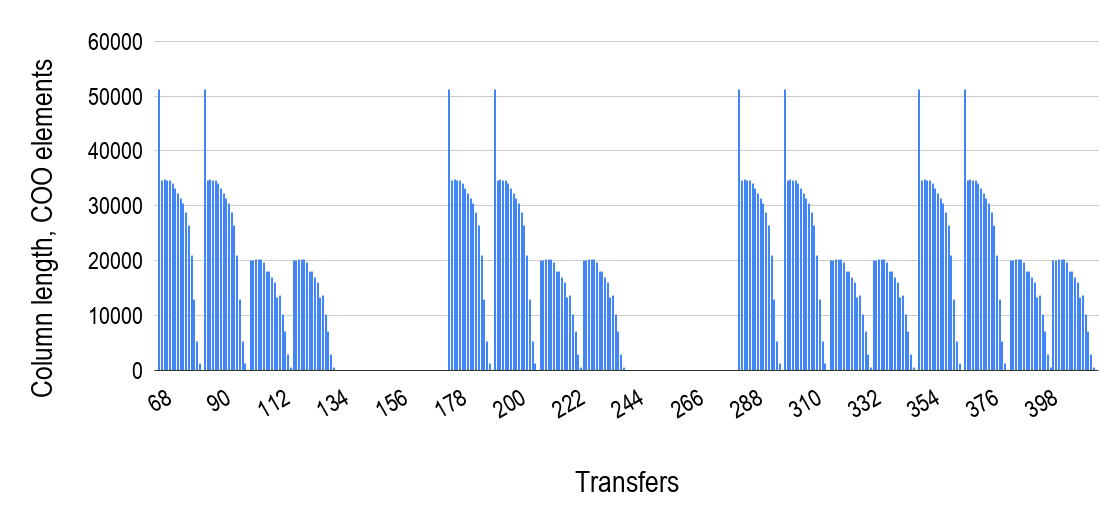
\includegraphics[width=1.0\textwidth]{figures/chapter-3/communication-pattern.png}
  \caption{A part of \textit{cube-64} communication pattern} \label{fig:communication-pattern}
\end{figure}


According to the \textit{accumulator} concept, described in section \ref{sec:accumulator-approach}, the main changes take place only on the client side and, hence, the server side remains unchanged which follows the original idea of the least code modifications. Code listing \ref{lst:bench:auxiliary-subroutines} represents an additional auxiliary class used for data accumulation. The pseudo-code of the benchmark client side is in listing \ref{lst:beanch:pseudocode}.\\ 


\begin{minipage}{\linewidth}
\begin{lstlisting}[language=python, caption={Pseudocode of an auxiliary \textit{Accumulator} class}, frame=single, label={lst:bench:auxiliary-subroutines}]
# problem_size - given Jacobian matrix size
# COO - compressed matrix coordinate format
class Accumulator:
	constructor(problem_size, acomm, acomm_id):
		private:
			N = problem_size; comm = acomm; id = acomm_id
			signal = [encode("add_to_jacobian"), id]
			is_allocated = false; is_non_blocking_op_called = false
			send_buffer = []
			factor = int(read_enviroment_variable("CNUT_ACC_SIZE"))
			if factor == None:
				factor = 1	
			permissible_size = factor * N	
		public: 
			accumulator = []
		
	def allocate_accumulator():
		if is_allocated == false:
			accumulator = allocate(2 * permissible_size, type(COO))			
			send_buffer = allocate(2 * permissible_size, type(COO))
			is_allocated = true

	def deallocate_accumulator():
		if is_allocated == true:
			deallocate(accumulator); deallocate(send_buffer)
			is_allocated = false
	
	def commit():
		if accumulator.size > permissible_size:
			swap(accumulator.pointer, send_buffer.pointer)
			if is_non_blocking_op_called == true:
				MPI_Wait()
			# perform 3-way handshake
			MPI_Send(signal, 2, int, comm.head, comm)
			# send data
			MPI_Ibcast(send_buffer.size, 1, int, comm.head, comm)
			MPI_Ibcast(send_buffer.data, send_buffer.size, COO, comm.all, comm)
			is_non_blocking_op_called = true
			accumulator.content.reset("to_beginning")
					
	def finalize():
		if is_non_blocking_op_called == true:
			MPI_Wait()
		MPI_Send(signal, 2, int, comm.head, comm)
		MPI_Bcast(accumulator.size, 1, int, comm.head, comm)
		MPI_Bcast(accumulator.data, accumulator.size, COO, comm.all, comm)
		is_non_blocking_op_called = false
		accumulator.content.reset("to_beginning")
\end{lstlisting}
\end{minipage}




\begin{minipage}{\linewidth}
\begin{lstlisting}[language=python, caption={Pseudocode of a modified client side of the benchmark}, frame=single, label={lst:beanch:pseudocode}]
# GIVEN PARAMETERS:
# acomm - the athlet communicator
# acomm_id - athlet identification number 
# N - problem size
# recording - data structure that holds a recorded communication pattern
# COO - compressed matrix coordinate format

if global_counter != 0:
	container = Accumulator.constructor(N, acomm, acomm_id)
	container.allocate_accumulator()
	++global_counter
	file = open("benchmark_results.txt", "w")

for column in recording:

	time_start = MPI_Wtime()
	
	# charge accumulator
	for i in range(column.length):
		element = generate_random_coo_element()		
		container.accumulator.add(element)

	# instantiate non-blocking data broadcast
	
		container.commit()
	time_end = MPI_Wtime() - time_start
	file.write(column.length, time_end)
	
# transfer the remainder and synchronize
time_start = MPI_Wtime()
	container.finalize()
time_end = MPI_Wtime() - time_start
file.write(column.length, time_end)


\end{lstlisting}
\end{minipage}


